\section{From Online Learning to Convex Optimization and Machine Learning}
\label{section:applications}

\begin{algorithm}[t]
\caption{SGD algorithm based on KT potential \label{algorithm:kt-sgd}}
\begin{algorithmic}[1]
{
\STATE{Initialize $\Wealth_0 \leftarrow 1$ and $\theta_0 \leftarrow 0$}
\FOR{$t=1,2,\dots,T$}
\STATE{Set $x_t \leftarrow \Wealth_{t-1} \tfrac{\theta_{t-1}}{t} $}
\STATE{Select an index $j$ at random from $\{1,2,\dots,N\}$ and compute $g_t \in \partial \ell_j(x_{t-1})$}
\STATE{Update $\theta_t \leftarrow \theta_{t-1}-g_t$ and $\Wealth_t \leftarrow \Wealth_{t-1} - \langle g_t, x_t \rangle$}
\ENDFOR
\STATE{Output $\overline{x}_T=\tfrac{1}{T}\sum_{t=1}^T x_t$}
}
\end{algorithmic}
\end{algorithm}

The results in Section~\ref{sec:algos} immediately implies new algorithms and
results in convex optimization and machine learning. See \cite{Orabona-2014} for more results.

\textbf{Convex Optimization.} 
Consider an emprical risk minimization problem of the form
%
\begin{equation}
\label{equation:objective-function}
\widehat{F}(w) = \frac{1}{N} \sum_{i=1}^N \ell_t(w),
\end{equation}
%
where $\ell_t$ is convex and $w \in \R^d$.\footnote{The algorithm can also be
implemented and analyzed with kernels~\citep{Orabona-2014}.} It is immediate to
transform Algorithm~\ref{algorithm:hilbert-space-olo} into a \ac{SGD} algorithm
for this problem. In Algorithm~\ref{algorithm:kt-sgd}, $\partial\ell_t(x)$
denotes the subgradient set of $\ell_t$ at a point $x$.  We assume that the
norm of the subgradient of $\ell_t$ is bounded by $1$.

Beside the simplicity of the algorithm, its important property is that it
\emph{does not have a learning rate to be tuned}, yet it achieves the optimal
convergence rate. If $\widehat{w} = \argmin_w \widehat{F}(w)$ is the optimal
solution of~\eqref{equation:objective-function}, the following theorem states
the rate of convergence.
%
\begin{theorem}
After $T$ iterations of Algorithm~\ref{algorithm:kt-sgd}, $\overline{w}_T$ is
an approximate minimizer of the function \eqref{equation:objective-function}:
\[
\Exp\left[\widehat{F}(\overline{w}_T)\right] - \widehat{F}(\widehat{w}) \leq \tfrac{\norm{\widehat{w}}}{\sqrt{T}} \sqrt{\log(1+4 T^2 \norm{\widehat{w}}^2)} +\tfrac{1}{T} \; .
\]
\end{theorem}
%
Note that in the above theorem, $T$ can be larger (multiple epochs) or smaller
than $N$.

\textbf{Machine Learning.} In a machine learning view, the minimization of a
function \eqref{equation:objective-function} is just a proxy to minimize the
\emph{true risk} over an unknown distribution. For example, $\ell_t(w)$ can be
a regression loss, e.g. the logistic loss, over samples $(x_t, y_t)$. That is,
$\ell_t(w)=\ell(w,x_t,y_t)$. A common approach to have a small
risk on the test set is to minimize a regularized objective function:
%
\begin{equation}
\label{eq:reg_logloss}
\widehat{F}^{\text{Reg}}(w) = \lambda \norm{w}^2 + \frac{1}{N} \sum_{i=1}^N \ell(w,x_t,y_t) \; .
\end{equation}
%
This problem is strongly convex, so there are very efficient methods to
minimize it, hence we can assume to be able to get the minimizer of
$\widehat{F}^{\text{Reg}}$ with arbitrary high precision. Yet, this is not
enough. In fact, we are rarely interested in the value of the objective
function, rather we are interested in the \emph{true risk} of a solution $w$,
that is $\Exp[\ell(w,X,Y)]$ where $X,Y$ comes from the unknown distribution
from which we sample the training and test points.  Hence, in order to get a
good performance we have to select a good regularization parameter. In
particular, from \cite{Sridharan-Shalev-Shwartz-Srebro-2009} we get
\[
\Exp[\ell(\widehat{w},X,Y)] - \Exp[\ell(w^*,X,Y)] \le O(\lambda \norm{w^*}^2 + \tfrac{1}{\lambda N}),
\]
where $w^*=\argmin_w \Exp[\ell(w,X,Y)]$.  From the above bound, it is clear
that the optimal value of $\lambda$ depends on the $\norm{w^*}$ that is
unknown. We would like to stress that this is not just a theoretical problem:
Any practictioner knows how painfull it is to find the right regularization for
the problem at hand.  Assuming to know $\norm{w^*}$, we could set $\lambda =
O(1/(\norm{w^*} \sqrt{N}))$ to achieve
%
\begin{equation}
\label{equation:optimal-rate}
\Exp[\ell(\widehat{w},X,Y)] - \Exp[\ell(w^*,X,Y)] \le O\left(\tfrac{\norm{w^*}}{\sqrt{N}}\right) \; .
\end{equation}

Using again Algorithm~\ref{algorithm:kt-sgd} with only one pass over the
dataset, we get almost the same guarantee \eqref{equation:optimal-rate}
\emph{without tuning any parameters, learning rates, regularization parameters,
etc.}
%
\begin{theorem}
Shuffle the dataset and do only one pass over the training set, using
$\ell_t(w)=\ell(w,x_t,y_t)$.  Algorithm~\ref{algorithm:kt-sgd}
satisfies
$$
\Exp[\ell(\overline{w}_N,X,Y)] - \Exp[\ell(w^*,X,Y)] \le \frac{\norm{w^*}}{\sqrt{N}} \sqrt{\log(1+4 N^2 \norm{w^*}^2)} + \tfrac{1}{N} \; .
$$
\end{theorem}
%
Comparing this guarantee to the one in \eqref{equation:optimal-rate}, we see
that, just paying a sub-logarithmic price, we obtain the optimal convergence
rate and we remove all the parameters.


\begin{figure}[t]
\centering
\subfigure{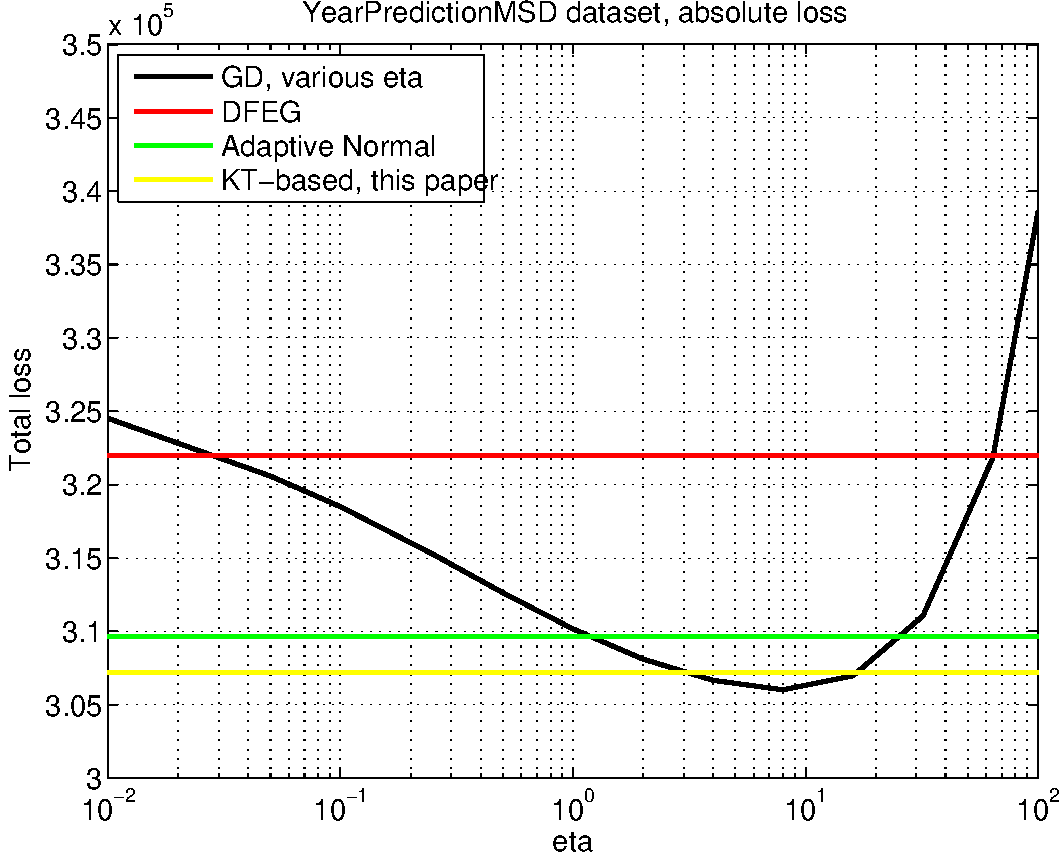
\includegraphics[width=0.32\textwidth]{../NIPS-2016-submission/figs/yearpredictionmsd_kt-crop.pdf}}
\subfigure{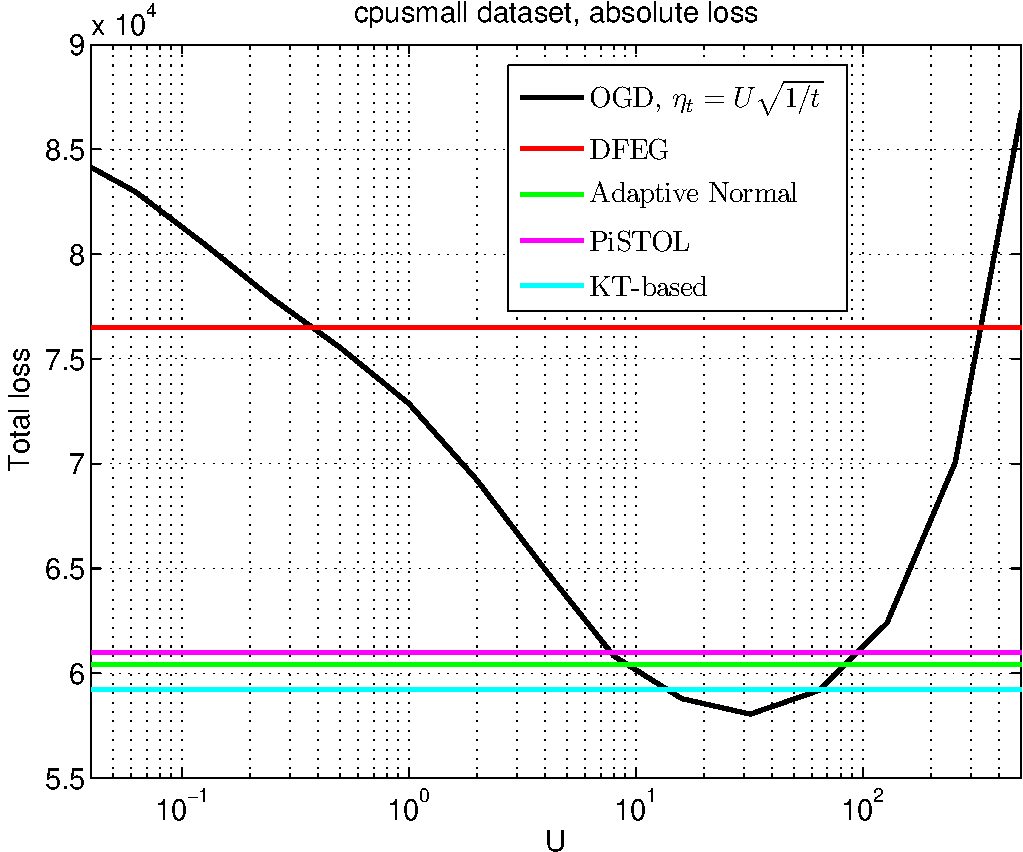
\includegraphics[width=0.32\textwidth]{../NIPS-2016-submission/figs/cpusmall_kt-crop.pdf}}
\subfigure{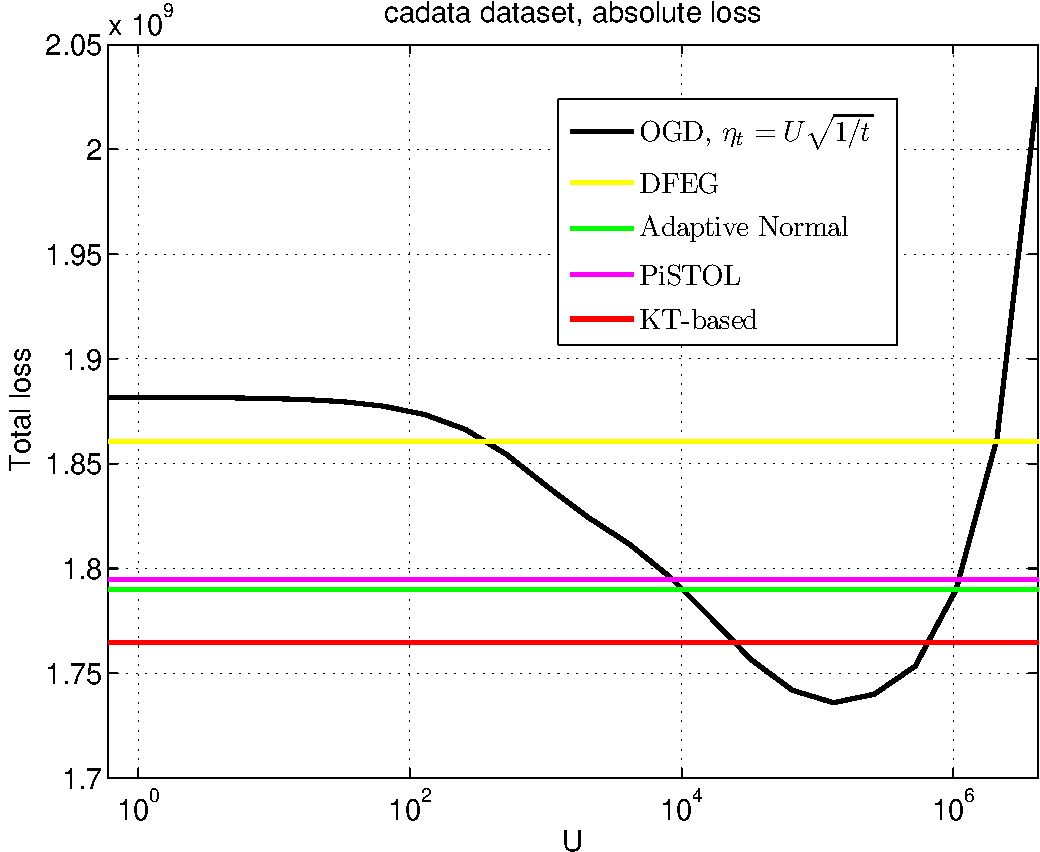
\includegraphics[width=0.32\textwidth]{../NIPS-2016-submission/figs/cadata_kt-crop.pdf}}
\caption{\footnotesize{Total loss versus learning rate parameter of \ac{OGD} (in log scale), compared with parameter-free algorithms DFEG~\cite{Orabona-2013}, Adaptive Normal~\cite{McMahan-Orabona-2014}, PiSTOL~\cite{Orabona-2014} and Algorithm~\ref{algorithm:kt-sgd}.}}
\label{fig:exp_olo}
\end{figure}
